\chapter{Environment Description}
\label{cha:env_description}



\section{arena description}


This section describes the simulated environment and agent in detail. The environment is a 3D simulation of a physical arena at the ScaDS.AI research facility. The simulated arena consists of a rectangular platform with enclosing walls. Simulated light sources illuminate the platform from above.
The goal of our agent is to complete tracks in the arena by traversing the track's goals in order. Each goal consists of 2 cuboid pillars of the same colour. The pillars are coloured red or blue. The goals' colours alternate in the track. The distance between the pillars is fixed and the same for all goals. The positions of the goals depends on the episode's track. The tracks are grouped by the difficulty settings easy, medium and hard. 

The tracks in the easy setting contain 3 goals that are positioned on the arena's center line with even distances between them. The medium setting contains 3 goals that are shifted on the center line towards the arena's walls. The hard setting contains 3 goals that are shifted on the center line towards the arena's walls, resulting in a zig-zag pattern. The zig-zag pattern is the most challenging for the agent to navigate, as it requires the agent to turn sharply to pass the goals. One track from each difficulty setting is shown in figure \ref{fig:track_difficulty_settings}. The tracks in each setting are structurally very similar to each other. They differ in goal coloring and the orientation of the shift from the center line.


\begin{figure}
    \centering
    \subfigure[Easy]{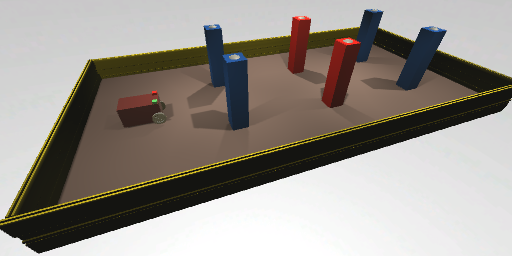
\includegraphics[width=0.3\textwidth]{Bilder/latex_images/evaluation_easy.png}}\qquad
    \subfigure[Medium]{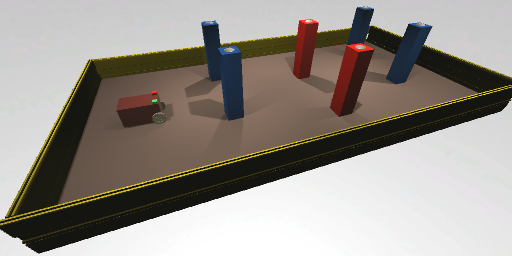
\includegraphics[width=0.3\textwidth]{Bilder/latex_images/evaluation_medium.png}}\qquad
    \subfigure[Hard]{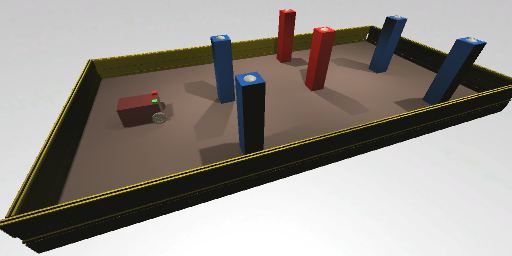
\includegraphics[width=0.3\textwidth]{Bilder/latex_images/evaluation_hard.png}}\\
    \caption{Example evaluation tracks for each difficulty setting.}
    \label{fig:track_difficulty_settings}
\end{figure}
% the images are generated with image_printer.py


There are three light settings for the environment, bright, standard and dark. The different light settings are achieved by varying the light intensities of the light sources above the arena and changing the horizon in the agent's camera.

\begin{figure}
    \centering
    \subfigure[Arena Bright]{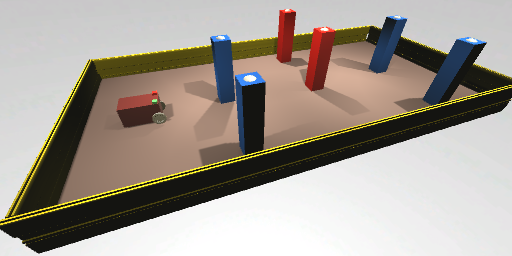
\includegraphics[width=0.3\textwidth]{Bilder/latex_images/light_setting_bright_arena.png}}\qquad
    \subfigure[Arena Standard]{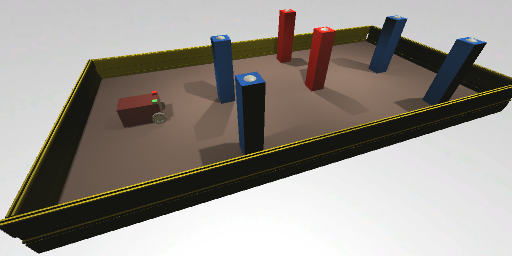
\includegraphics[width=0.3\textwidth]{Bilder/latex_images/light_setting_standard_arena.png}}\qquad
    \subfigure[Arena Dark]{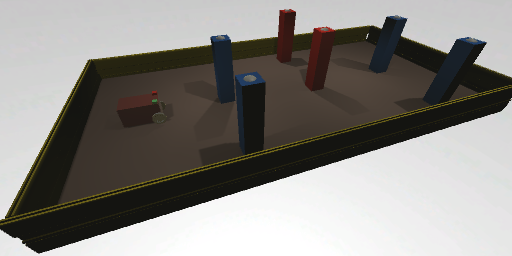
\includegraphics[width=0.3\textwidth]{Bilder/latex_images/light_setting_dark_arena.png}}\\
    \subfigure[Agent Bright]{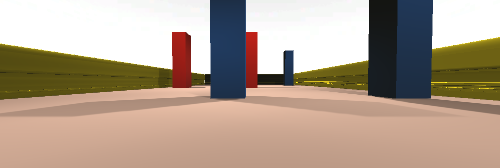
\includegraphics[width=0.3\textwidth]{Bilder/latex_images/light_setting_bright_pov_no_preprocessing.png}}\qquad
    \subfigure[Agent Standard]{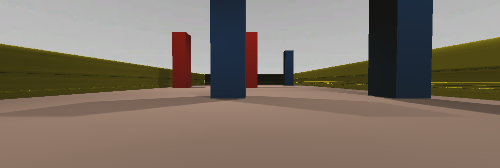
\includegraphics[width=0.3\textwidth]{Bilder/latex_images/light_setting_standard_pov_no_preprocessing.png}}\qquad
    \subfigure[Agent Dark]{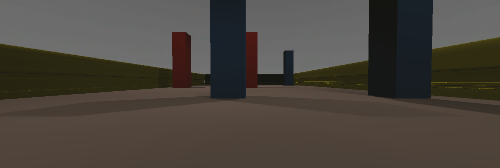
\includegraphics[width=0.3\textwidth]{Bilder/latex_images/light_setting_dark_pov_no_preprocessing.png}}\\
    \caption{Arena and agent camera at different light settings.}
    \label{fig:track_light_settings}
\end{figure}



\section{Agent Description}

The agent is modeled after the NVIDIA JetBot, a small robot designed for educational purposes. The NVIDIA JetBot is equipped with a camera and a differential drive system. The agent's camera is mounted on the JetBot's front and captures the arena from the JetBot's perspective. The camera captures the arena in a 2D image format. 
There are two versions of the JetBot agent in the simulation, the DifferentialJetBot and the FourWheelJetBot. The DifferentialJetBot has two driving wheels at the front and a ball supporting it at the back. The FourWheelJetBot has 2 steering driving wheels at the front and two non-driving wheels in the back. The DifferentialJetBot steers by applying different torques to the two front wheels. The FourWheelJetBot steers by turning the front wheels in the desired direction and applyig equal torques to both wheels.
The FourWheelJetBot was used in the work by \autocite{maximilian}. The DifferentialJetBot was developed to match the physical NVIDIA JetBot more closely. The two JetBot designs are shown in figure \ref{fig:jetbots}.

\begin{figure}
    \centering
    \subfigure[Nvidia JetBot Photo]{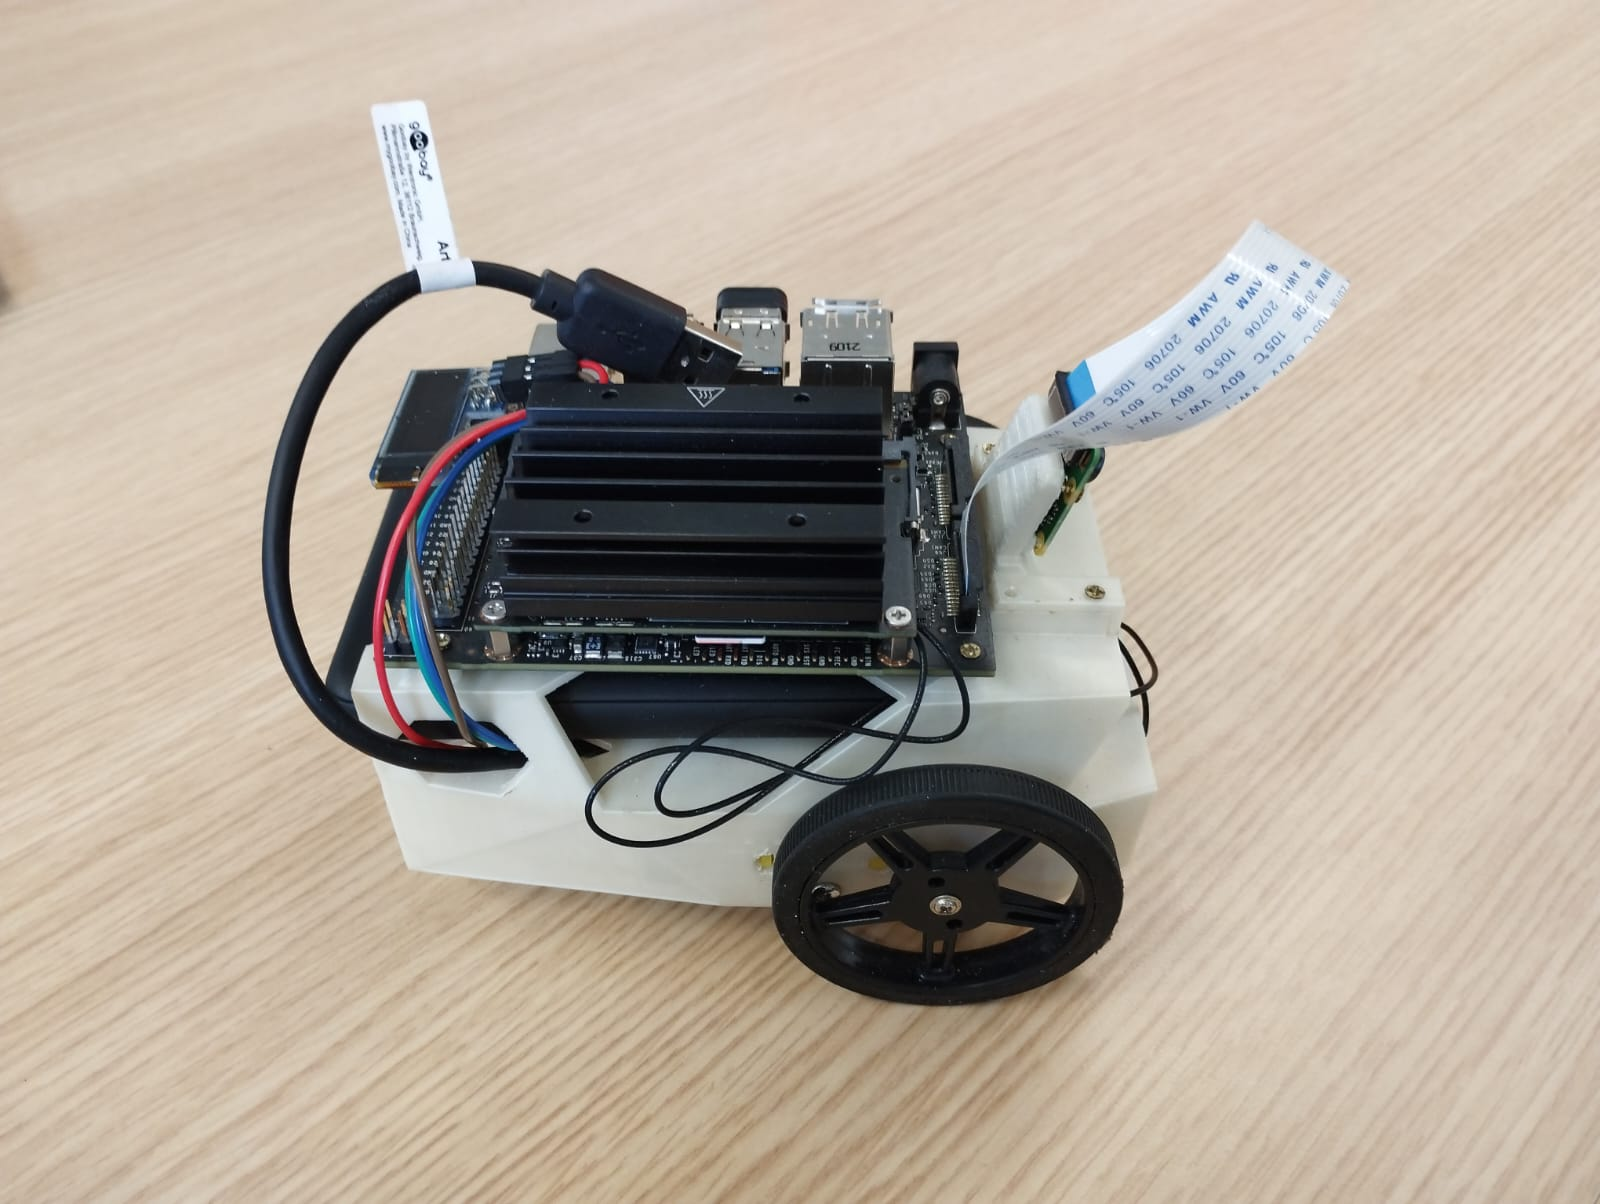
\includegraphics[width=0.3\textwidth]{Bilder/JetBotImages/NvidiaJetBot.jpeg}}\qquad
    \subfigure[DifferentialJetBot]{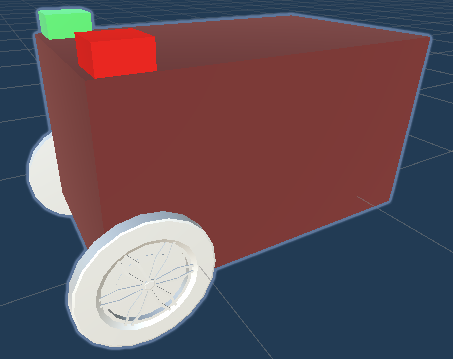
\includegraphics[width=0.3\textwidth]{Bilder/JetBotImages/DifferentialJetBot.PNG}}\qquad
    \subfigure[FourWheelJetBot]{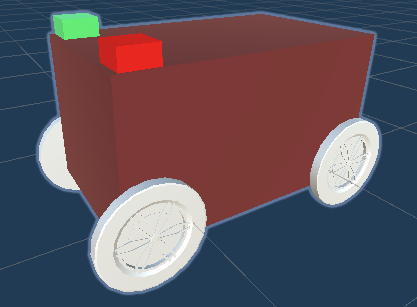
\includegraphics[width=0.3\textwidth]{Bilder/JetBotImages/FourWheelJetBot.PNG}}\qquad
    \caption{Original Nvidia JetBot and simulated JetBot Desgins}
    \label{fig:jetbots}
\end{figure}


\section{Episode Design}

An episode represents one attempt of the agent at solving a track in the environment. Each episode consists of a series of steps starting from the initial position. The agent interacts with the environment in each step. The environment is simulated in Unity during each step. This includes things like agent movement, collision detection and reward calculation.

The duration of each step is defined by the environment settings. There are two destinct modes for the step durations. The first mode is the fixed timestep mode. In this mode the duration of each step is fixed and defined by the environment parameter $fixedTimestepsLength$. The second mode is the variable timestep mode. In this mode each step lasts until the environment receives the next action from the agent.

\label{time_limit}The episodes are terminated based on the agent's interactions with the environment. Episodes are terminated when the agent reaches the finish line or a timeout is reached. The timeout is defined by a fixed timelimit of 20 seconds which is increased by further 20 seconds for each passed goal. The timelimit is necessary to terminate episodes where the agent does not reach the finish line, due to the policy's learned behaviour or collisions. 

Collisions of the agent with the goal posts and the arena walls are detected by the environment. The environment parameter $collisionMode$ defines how the agent's collisions are handled. The $collisionMode$ can take 5 different values described in table \ref{fig:collision_modes}.

\begin{figure}
    
    \begin{center}
    \begin{tabular}{|| p{0.2\linewidth} | p{0.35\linewidth} | p{0.35\linewidth} ||} 
        \hline
        collisionMode & \makecell{Behaviour upon Collision} & Reasoning \\ [0.5ex] 
        \hline\hline
        unrestricted & Negative reward is given for each frame with collision.  This can result in multiple penalties given during a single step. & Default behaviour \\ 
        \hline
        oncePerTimestep & Negative reward for collisions is given only once per step. & Limits the negative reward caused by a collision in a step. \\
        \hline
        oncePerEpisode & Negative reward for collision is only given once  per episode per object. & Limits the negative reward caused by ongoing collisions. \\
        \hline
        terminate  & Episode is terminated instantly. & The early termination could speed up the neural network training. \\
        \hline
        ignore  & Collisions are ignored, no negative reward is given. & The agent might learn to avoid collisions based on other rewards. \\
        \hline
    \end{tabular}
    \end{center}
    \caption{Collision Modes}
    \label{fig:collision_modes}
\end{figure}



time-limit, episode termination, step-function, Collisions, rewards

time limit explain here

explain the spawn positions here?
(currently in MethodsTrainAlgorithm.tex)


% success is now defined as passing all three goals  (without necessarily reaching the finish line)
% this was done as the agent sometimes learns to move back and forth in front of the finish line


\section{Reward Function}



Previous sections introduced the composite reward function. The composite reward function consists of a weighted sum of individual reward functions. The individual reward functions are designed to encourage the agent to learn the desired behaviour. The goal is to achieve an agent that completes the parcour without collisions, this is encapsulated in the event reward function. However the event reward function is a very sparse signal, which makes it hard for the agent to learn. The other individual reward functions are designed to not be sparse, however some of these functions are not enough to guide the agent to the desired behaviour alone, such as the orientation reward.
It is important to find appropriate weights of the individual reward functions for the composite reward function. We are conducting experiments to analyse the usefullness of the individual reward functions. We analyse if the agent is capable of learning the behaviour encouraged by the reward function.

see \ref{table:reward_functions_behaviour}


\begin{table}
    
\caption{Training runs with different reward functions alone (all coefficients 0 except the one of the reward function)}
\begin{center}
\begin{tabular}{|| c | c | c | c ||} 
    \hline
    \makecell{function \\ name} & encouraged behaviour & learned behaviour  & \makecell{expected behaviour \\ learned?} \\ [0.5ex] 
    \hline\hline
    \makecell{event \\ reward} &  \makecell{agent drives through the parcour \\ without collisions} & \makecell{agent turns on the spot \\ continuously} & no \\ 
    \hline
    \makecell{distance \\ reward} & agent drives towards the next goal & agent drives towards the next goal & yes \\
    \hline
    \makecell{orientation \\ reward} & agent turns towards closest goal & \makecell{agent turns around on the spot \\ continuously} & no \\
    \hline
    \makecell{velocity \\ reward}  & full speed ahead (no turning) & full speed ahead (no turning) & yes \\
    \hline
\end{tabular}
\end{center}
\label{table:reward_functions_behaviour}
\end{table}


